\documentclass{article}

\usepackage{iclr2027_conference,times}
\usepackage{amsmath,amssymb}
\usepackage{booktabs}
\usepackage{graphicx}
\usepackage{subcaption}
\usepackage{microtype}
\usepackage{hyperref}
\usepackage{url}

\graphicspath{{figures/}}

\title{Beyond Permutation Symmetry: Width and Scaling in Linear Mode Connectivity}

% Authors are hidden by the ICLR style while \iclrfinalcopy remains commented.
\author{Anonymous authors\\Paper under double-blind review}

% \iclrfinalcopy

\newcommand{\barrier}{\mathcal{B}}
\newcommand{\loss}{\mathcal{L}}

\begin{document}

\maketitle

% Keep the anonymous submission title block, but suppress the review line-number
% overlay in this reading draft. Remove this line for the numbered submission PDF.
\iclrfinaltrue

\begin{abstract}
Permutation symmetry is often used to explain why independently trained neural
networks appear separated under linear interpolation.  We test where that
explanation is exact, where it depends on width, and whether a larger symmetry
class is needed.  On XOR, exhaustive enumeration gives an oracle over all
hidden-unit permutations.  Minimal-width ReLU networks provide concrete pairs
for which every permutation retains a loss barrier, ruling out permutation
search failure in this setting.  Increasing width rapidly lowers the oracle
barrier, while a separate nonlinear-path experiment exhibits a sharp change
between widths two and three, separating symmetry alignment from
representational slack.  We then exploit positive scaling symmetry and propose
a scale-aware extension of differentiable Sinkhorn re-basing.  Starting from
the oracle permutation and optimizing only scales reduces the mean XOR barrier
from $0.357$ to $0.247$, $0.111$ to $0.025$, and $0.023$ to $0.005$ at hidden
widths $3$, $5$, and $7$, respectively, and never worsens a pair.  A
shared-training experiment shows that permutation alignment becomes harder as
training trajectories diverge, and experiments on VGG networks trained on
CIFAR-10 show that adding scale improves over permutation-only alignment in all
four tested architectures.  These results refine the one-basin picture:
permutation explains part of linear compatibility, width supplies additional
slack, and positive scaling is a practically relevant exact symmetry beyond
permutation.
\end{abstract}

\section{Introduction}

Neural networks trained from different random initializations usually occupy
distant points in parameter space, and the straight line between their weights
often crosses a region of high loss.  This observation appears to suggest that
stochastic gradient descent (SGD) finds distinct basins.  Yet neural-network
parameterizations are highly non-identifiable.  Reordering hidden units or
channels, with the inverse reordering applied to the next layer, preserves the
represented function.  Consequently, a barrier between two raw parameter
vectors may reflect an arbitrary choice of representative rather than genuine
geometric separation.

The one-basin modulo permutation hypothesis makes this intuition precise: most
SGD solutions may admit functionally equivalent permutations that are linearly
mode connected~\citep{entezari2021role}.  Explicit alignment methods have made
this hypothesis operational.  Git Re-Basin substantially reduces barriers for
MLPs and convolutional networks and obtains essentially barrier-free
interpolation in several sufficiently wide settings~\citep{ainsworth2023git}.
However, residual barriers remain for more difficult architectures and smaller
widths.  Such failures have two incompatible explanations: the search method
may miss a good permutation, or no good permutation may exist.  Modern networks
have combinatorially large permutation groups, so standard experiments cannot
separate these possibilities.

We use a small setting in which the ambiguity disappears.  For one-hidden-layer
XOR networks, every permutation can be evaluated exactly.  This controlled
test reveals trained pairs for which permutation is genuinely insufficient,
and a width sweep shows how quickly the failure weakens as redundant units are
added.  We complement the linear test with nonlinear path optimization at
widths two and three.  This distinguishes two mechanisms that can otherwise be
conflated: selecting a better representative using exact symmetries, and using
extra model capacity to move through a broader low-loss set.

The failure of an exhaustive permutation search motivates a larger exact
symmetry class.  ReLU networks are invariant to positive rescaling of a hidden
unit when the outgoing weight is inversely rescaled.  We incorporate these
continuous degrees of freedom into Sinkhorn re-basing~\citep{guerrero2023rebasin}
and also study a cleaner oracle protocol: first choose the best exhaustive
permutation, then optimize scales while freezing that permutation.  The latter
isolates the benefit of scaling from improvements in permutation search.

Our contributions are:
\begin{itemize}
    \item An exhaustive XOR counterexample showing that nonzero barriers can
    remain after the best possible permutation, together with a width sweep
    demonstrating that the oracle barrier collapses as redundancy grows.
    \item A nonlinear-connectivity comparison between widths two and three,
    showing that one extra hidden unit can change path connectivity even when
    permutation-based LMC remains imperfect.
    \item A scale-aware Sinkhorn parameterization and an oracle
    permutation-plus-scale experiment.  Scale refinement improves or preserves
    the barrier for all $67$ tested XOR pairs and produces the largest gains at
    widths five and seven.
    \item A training-stage analysis on VGG16 and a realistic validation on
    VGG11/13/16/19 trained on CIFAR-10.  The former links alignment difficulty
    to training divergence; the latter shows consistent gains from scale beyond
    permutation-only alignment.
\end{itemize}

\section{Background and Related Work}

\paragraph{Connectivity and interpolation barriers.}
For endpoints $\theta_A$ and $\theta_B$, linear interpolation is
$\theta(t)=(1-t)\theta_A+t\theta_B$.  Following prior work, for a scalar
criterion $C$ (loss or classification error) we measure the excess above the
linear interpolation of endpoint values:
\begin{equation}
\barrier(\theta_A,\theta_B;C)=
\max_{t\in[0,1]}\left[C(\theta(t))-
(1-t)C(\theta_A)-tC(\theta_B)\right].
\label{eq:barrier}
\end{equation}
The maximum is approximated on a dense grid.  Low-barrier curved paths between
independent solutions are widespread~\citep{draxler2018essentially,garipov2018loss},
but curved connectivity is weaker than linear mode connectivity (LMC): the path
may avoid a region crossed by the straight segment.  Shared-initialization
experiments further show that solutions become linearly stable to SGD noise
early in training~\citep{frankle2020linear}.

\paragraph{Why linear connectivity matters.}
A curved connection establishes geometric connectedness, but a straight path
is the relevant object for weight averaging.  Averaging checkpoints from one
training trajectory can improve generalization by favoring a wider region of
parameter space~\citep{izmailov2018averaging}, and averaging related fine-tuned
models can outperform the individual endpoints without ensemble-time
cost~\citep{wortsman2022model}.  Independent models are harder: if their hidden
features use incompatible coordinates, the midpoint mixes unrelated units and
can be unusable even when both endpoints are accurate.  Re-basing seeks a
functionally equivalent coordinate system before averaging.  Our results focus
on the prerequisite---a low-barrier segment---rather than claiming that the
midpoint necessarily improves endpoint accuracy.  This distinction matters
because a symmetry transformation can repair compatibility while providing no
new predictive information by itself.

\paragraph{Permutation re-basing.}
For a ReLU MLP block $f(x)=W_2\sigma(W_1x)$ and a permutation matrix $P$,
\begin{equation}
(W_2P^\top)\sigma(PW_1x)=W_2\sigma(W_1x).
\label{eq:perm}
\end{equation}
The same action reorders channels in convolutional networks.  Weight matching
finds layerwise permutations that reduce Euclidean distance, activation
matching aligns representations on data, and differentiable methods optimize
soft assignments~\citep{ainsworth2023git,guerrero2023rebasin}.  REPAIR shows
that correcting activation statistics can further improve interpolation after
permutation~\citep{jordan2023repair}.  These successes support a symmetry-aware
view of loss landscapes, but a residual barrier obtained by a heuristic cannot
establish that the symmetry class itself is insufficient.

\paragraph{Positive scaling symmetry.}
Positive homogeneity, $\sigma(cz)=c\sigma(z)$ for $c>0$, yields a second exact
symmetry.  With $D$ positive diagonal,
\begin{equation}
(W_2D^{-1})\sigma(DW_1x)=W_2\sigma(W_1x).
\label{eq:scale}
\end{equation}
Permutation and scale therefore form a monomial action $M=PD$.  Unlike a
permutation, scaling moves a representative continuously and can substantially
change its Euclidean relation to a second model.  Our question is not whether
scaling changes either endpoint function---it does not---but whether it selects
representatives whose straight-line interpolation is better behaved.

\section{Scale-Aware Alignment}
\label{sec:method}

Sinkhorn re-basing replaces a hard layerwise permutation by a differentiable,
approximately doubly stochastic matrix
\begin{equation}
S_\ell=\operatorname{Sinkhorn}(Z_\ell/\tau),
\end{equation}
where $Z_\ell$ is an unconstrained score matrix and $\tau$ is a temperature.
Repeated row and column normalization of $\exp(Z_\ell/\tau)$ permits gradient
optimization through the alignment.  After optimization, the soft matrix is
projected to a hard permutation using linear assignment.

We augment each hidden layer with learnable log-scales $u_\ell$:
\begin{equation}
D_\ell=\operatorname{diag}(e^{u_\ell}),\qquad
M_\ell=S_\ell D_\ell.
\label{eq:monomial}
\end{equation}
On the output coordinates of layer $\ell$ we apply $S_\ell D_\ell$; on the
input coordinates of the next layer we apply the compensating
$D_\ell^{-1}S_\ell^\top$.  Once $S_\ell$ is projected to a permutation, this is
the exact function-preserving monomial transformation in
Eqs.~\ref{eq:perm}--\ref{eq:scale}.  During soft optimization, the transpose is
the usual differentiable Sinkhorn approximation rather than an exact inverse.

The variables are optimized on real data using midpoint interpolation loss:
\begin{equation}
J=\loss\!\left(\tfrac12\theta_A+\tfrac12 M(\theta_B)\right)
+\lambda\sum_\ell\lVert u_\ell\rVert_2^2.
\label{eq:objective}
\end{equation}
The regularizer biases the solution toward identity scaling and limits the
otherwise unbounded scale gauge.  We use two variants.  \emph{Joint
permutation+scale} optimizes $Z_\ell$ and $u_\ell$ together.  \emph{Scale
refinement} first obtains hard permutations, freezes them, and optimizes only
$u_\ell$.  The second variant can be applied after any permutation method and,
when initialized with an exhaustive oracle, cleanly attributes any improvement
to scale rather than a changed correspondence.

\subsection{Why an exact symmetry changes the interpolation path}

Although scaling leaves the transformed endpoint function unchanged, it does
not leave the functions in the interior of a straight parameter-space path
unchanged.  This distinction is the source of its utility.  Consider one hidden
ReLU unit with incoming weight $w$ and outgoing weight $v$, and suppose for
illustration that the activation pattern stays fixed along the segment.  At the
midpoint between unit $(w_A,v_A)$ and a scaled representative
$(d w_B,v_B/d)$, its locally linear contribution contains
\begin{equation}
\frac{1}{4}\left[v_A w_A+v_B w_B+d\,v_A w_B+d^{-1}v_B w_A\right]^\top x.
\label{eq:cross-terms}
\end{equation}
The first two terms are determined by the endpoints, but the two cross terms
depend on $d$.  Positive scaling can therefore balance the incompatible
incoming and outgoing features that are mixed by interpolation.  With multiple
units and changing ReLU gates the expression is piecewise rather than globally
linear, but the same mechanism remains: choosing a different representative on
the symmetry orbit changes cross-model interactions while preserving both
endpoint functions.

This also clarifies the different roles of width and symmetry.  For a fixed
width, permutation provides a finite orbit and scaling adds continuous
directions within each permutation cell.  Increasing width does more than
enlarge that orbit: it changes the function class and can distribute a feature
across redundant units, making both linear matching and curved motion easier.
The experiments below are designed to observe these effects separately rather
than treating every improvement as a better permutation search.

\section{Experimental Design}
\label{sec:design}

\paragraph{XOR endpoints.}
We train one-hidden-layer ReLU MLPs on the four XOR inputs with binary labels,
using full-batch SGD and binary cross-entropy.  Models are initialized uniformly
in $[-0.5,0.5]$, trained for at most $5000$ epochs, and retained only when they
reach $100\%$ accuracy and low endpoint loss.  For width $h$, all $h!$ hidden
unit permutations are enumerated.  The best permutation minimizes the sampled
interpolation barrier, providing an exact oracle within permutation symmetry.
For scale-aware experiments, interpolation is evaluated at $61$ values of $t$.
We obtain $21$, $36$, and $10$ valid pairs at $h=3,5,7$.

\paragraph{Nonlinear paths.}
To distinguish linear alignment from broader connectivity, we optimize both
quadratic B\'ezier paths and polygonal chains between independently trained XOR
endpoints.  We begin with one trainable interior point and increase path
flexibility up to ten interior points.  The objective is the maximum loss over
$31$ sampled path locations.

\paragraph{Training-stage benchmark.}
For VGG16 on CIFAR-10, two branches share an initialization and the first $n$
of $N=200$ epochs, then train independently with different minibatch orders and
augmentations.  Later splits produce more closely related endpoints.  A known
random channel permutation is applied to one endpoint, and weight matching is
asked to undo the mismatch.  Because applying the inverse known permutation
recovers the original branch, each split has a reference alignment.  Repeating
weight matching with different layer-update orders measures search variability.

\paragraph{VGG validation.}
We evaluate fixed independently trained seed-0/seed-1 pairs of VGG11, VGG13,
VGG16, and VGG19 on CIFAR-10.  We compare raw interpolation, permutation-only
Sinkhorn, joint permutation+scale, and permutation followed by scale
refinement.  Alignment uses a deterministic calibration batch and minimizes
midpoint loss; final results use hard permutations and test-set interpolation.
Because each architecture is represented by one endpoint pair and method-wise
hyperparameters are selected separately, this experiment is a realistic
validation of the qualitative pattern, not a population estimate.

Additional optimization settings and reproducibility details appear in
Appendix~\ref{app:details}.

\section{Permutation Insufficiency and the Role of Width}
\label{sec:xor}

\subsection{An exhaustive counterexample}

At the minimal width $h=2$, only the identity and swap are valid permutations.
Several independently trained pairs retain a substantial barrier under both.
Figure~\ref{fig:xor-counterexample} shows representative cases.  Alignment
succeeds for seeds 2 and 4 because their parameters are nearly identical after
a swap.  In contrast, seeds 9 and 12 implement the same XOR labels and have
visually similar decision boundaries, yet their internal weights are not
related by either permutation and the barrier remains.  A second failure mode
occurs when perfect-accuracy solutions implement different boundaries away from
the four training inputs.  Since the search enumerates the full group, these
failures cannot be blamed on the permutation optimizer.  They form a concrete
counterexample to a universal permutation-only LMC claim for trained networks;
they do not contradict a claim restricted to sufficiently wide networks or to
``most'' solutions.

\begin{figure}[t]
    \centering
    \begin{subfigure}[t]{0.49\linewidth}
        \centering
        \includegraphics[width=\linewidth]{success.png}
        \caption{Successful pair: a swap makes the endpoints nearly identical.}
    \end{subfigure}
    \hfill
    \begin{subfigure}[t]{0.49\linewidth}
        \centering
        \includegraphics[width=\linewidth]{unsuccesfull_same_boundary.png}
        \caption{Failed pair: similar boundary, but neither permutation removes the barrier.}
    \end{subfigure}
    \caption{Exhaustive permutation alignment for width-$2$ XOR networks.
    Columns in each panel are interpolation points; top and bottom rows show raw
    and best-permuted interpolation.  Both endpoints classify all four XOR
    points correctly.}
    \label{fig:xor-counterexample}
\end{figure}

\subsection{Width lowers the oracle barrier}

Increasing width changes the result.  In the initial exhaustive sweep over
$h\in\{2,3,4,5\}$, the number of pairs maintaining $100\%$ accuracy along the
best-permuted interpolation rises steadily; at $h=5$, every evaluated pair
maintains perfect accuracy.  Perfect accuracy does not mean zero loss barrier:
midpoint confidence can still fall relative to the endpoints.

The larger scale-aware study quantifies this effect in loss.  Table
\ref{tab:xor-scale} shows that the oracle permutation barrier falls from $0.357$
at $h=3$ to $0.111$ at $h=5$ and $0.023$ at $h=7$.  Thus, even before scaling,
width supplies matching flexibility.  Practical Sinkhorn permutation search is
weaker than the oracle at all widths, illustrating why heuristic failure alone
cannot diagnose the absence of an alignment.

\begin{table}[t]
\caption{XOR loss barrier (mean $\pm$ standard deviation).  Oracle+scale first
selects the exhaustive best permutation, then optimizes only positive scales.
The final row counts pairs for which refinement is no worse than the oracle.}
\label{tab:xor-scale}
\centering
\small
\begin{tabular}{lccc}
\toprule
Method & $h=3$ & $h=5$ & $h=7$ \\
\midrule
No alignment & $0.780\pm0.610$ & $0.608\pm0.465$ & $0.331\pm0.184$ \\
Sinkhorn permutation & $0.444\pm0.325$ & $0.189\pm0.162$ & $0.063\pm0.044$ \\
Oracle permutation & $0.357\pm0.309$ & $0.111\pm0.118$ & $0.023\pm0.015$ \\
Joint permutation+scale & $0.428\pm0.380$ & $0.074\pm0.149$ & $0.009\pm0.009$ \\
Oracle+scale & $\mathbf{0.247\pm0.283}$ & $\mathbf{0.025\pm0.044}$ & $\mathbf{0.005\pm0.003}$ \\
\midrule
Oracle+scale $\leq$ oracle & $21/21$ & $36/36$ & $10/10$ \\
\bottomrule
\end{tabular}
\end{table}

\subsection{Nonlinear connectivity changes at width three}

Permutation-based LMC and general mode connectivity need not change at the same
width.  At $h=2$, extensive B\'ezier and polygonal searches find low-loss paths
only for essentially identical endpoints; additional bends do not recover
nontrivial connections.  At $h=3$, all studied endpoint pairs are connected by
low-loss paths.  Most are found directly; for one difficult pair, low-loss
paths through a third trained mode establish connectivity by concatenation.
Figure~\ref{fig:nonlinear-width} contrasts a width-$2$ failure with a width-$3$
success between models having different decision boundaries.

This is evidence about the paths found by the tested parameterizations, not a
topological impossibility theorem for width two.  Nevertheless, the sharp
empirical transition is informative: adding a single hidden unit provides
representational slack that permits a curved route even when the best straight
symmetry-aligned route can retain loss.  Width therefore affects connectivity
through more than an enlarged permutation group.

\begin{figure}[t]
    \centering
    \includegraphics[width=\linewidth]{unsuccesful_10-14_bezier_3bend.png}
    \vspace{-1ex}
    \includegraphics[width=\linewidth]{3hidden_xor_bezier.png}
    \caption{Nonlinear XOR paths.  \emph{Top:} a representative width-$2$
    pair for which optimizing a B\'ezier path does not remove the high-loss
    region.  \emph{Bottom:} at width $3$, a low-loss path connects endpoints
    with different decision boundaries.  The rows visualize predictions along
    the learned path.}
    \label{fig:nonlinear-width}
\end{figure}

\section{Scale Improves on the Permutation Oracle}
\label{sec:scale-results}

The decisive comparison in Table~\ref{tab:xor-scale} is between oracle
permutation and oracle+scale.  The hard assignment is identical in the two
conditions, so the improvements can only come from selecting a different
functionally equivalent scaling of the same endpoint.  Refinement reduces the
mean barrier by $31\%$ at $h=3$, $77\%$ at $h=5$, and $78\%$ at $h=7$.  It is
no worse on every one of the $67$ pairs.  This shows that positive scale is not
merely helping a relaxed optimizer discover a better permutation; it enlarges
the attainable set beyond the exhaustive permutation orbit.

Joint optimization is more mixed at the narrowest width.  It improves over the
permutation oracle on $9/21$, $29/36$, and $8/10$ pairs at widths $3$, $5$, and
$7$, respectively.  At $h=3$, its mean barrier ($0.428$) remains above the
oracle-permutation result ($0.357$), whereas at widths five and seven it beats
the oracle mean.  The difference between joint and oracle-refinement results
exposes an optimization gap: a richer symmetry class can contain better
representatives without a from-scratch solver reliably finding them.

Figure~\ref{fig:xor-profiles} shows the averaged interpolation profiles.  All
curves improve with width, but oracle scale refinement (green) is consistently
lowest.  At $h=7$, its mean maximum excess is only $0.005$, compared with
$0.023$ for the best permutation.  Scaling matters most once width has already
made useful correspondences available: it fine-tunes the balance of incoming
and outgoing weights without changing endpoint predictions.

\begin{figure}[t]
    \centering
    \begin{subfigure}[t]{0.32\linewidth}
        \includegraphics[width=\linewidth]{3h_xor.png}
    \end{subfigure}
    \begin{subfigure}[t]{0.32\linewidth}
        \includegraphics[width=\linewidth]{h5_xor.png}
    \end{subfigure}
    \begin{subfigure}[t]{0.32\linewidth}
        \includegraphics[width=\linewidth]{h7_xor.png}
    \end{subfigure}
    \caption{Mean XOR interpolation loss at widths $3$, $5$, and $7$: raw
    interpolation (gray), Sinkhorn permutation (orange), exhaustive oracle
    permutation (blue), joint permutation+scale (purple), and oracle
    permutation followed by scale refinement (green).  Exact barriers are in
    Table~\ref{tab:xor-scale}.}
    \label{fig:xor-profiles}
\end{figure}

\section{When Does Alignment Become Difficult?}
\label{sec:training-stage}

The shared-training construction provides a dynamic view.  Two VGG16 branches
are identical until the split, after which SGD noise makes them diverge.  A
random known permutation is then added to one endpoint.  Figure
\ref{fig:training-stage} plots test-error barrier against endpoint distance
before and after weight matching.  Late splits lie in the lower-left: their
endpoints remain close, the reference path already has low barrier, and weight
matching reliably removes the artificial mismatch.  Early splits lie farther
away and retain much larger barriers.

For every shared-split pair, the recovered alignment is at least as good as the
known inverse permutation and often better.  Repeating weight matching with
different layer-update orders produces small variability (the largest barrier
standard deviation is about $0.68$ percentage points for the $0/200$ split and
becomes negligible for late splits).  The trend is therefore not explained by
one unlucky search order.

Distance is informative but not sufficient.  The $4/196$ shared-split pair has
a test-error barrier of approximately $21.7$ percentage points near distance
$28$, whereas the independently initialized pair after matching has a barrier
of $34.1$ points at a comparable distance.  The experiment suggests that
weight similarity is a useful proxy when trajectories share substantial
history, but ceases to characterize linear compatibility once their learned
representations diverge.  This motivates optimizing interpolation loss within
a broader symmetry orbit, as in Section~\ref{sec:method}.

\begin{figure}[t]
    \centering
    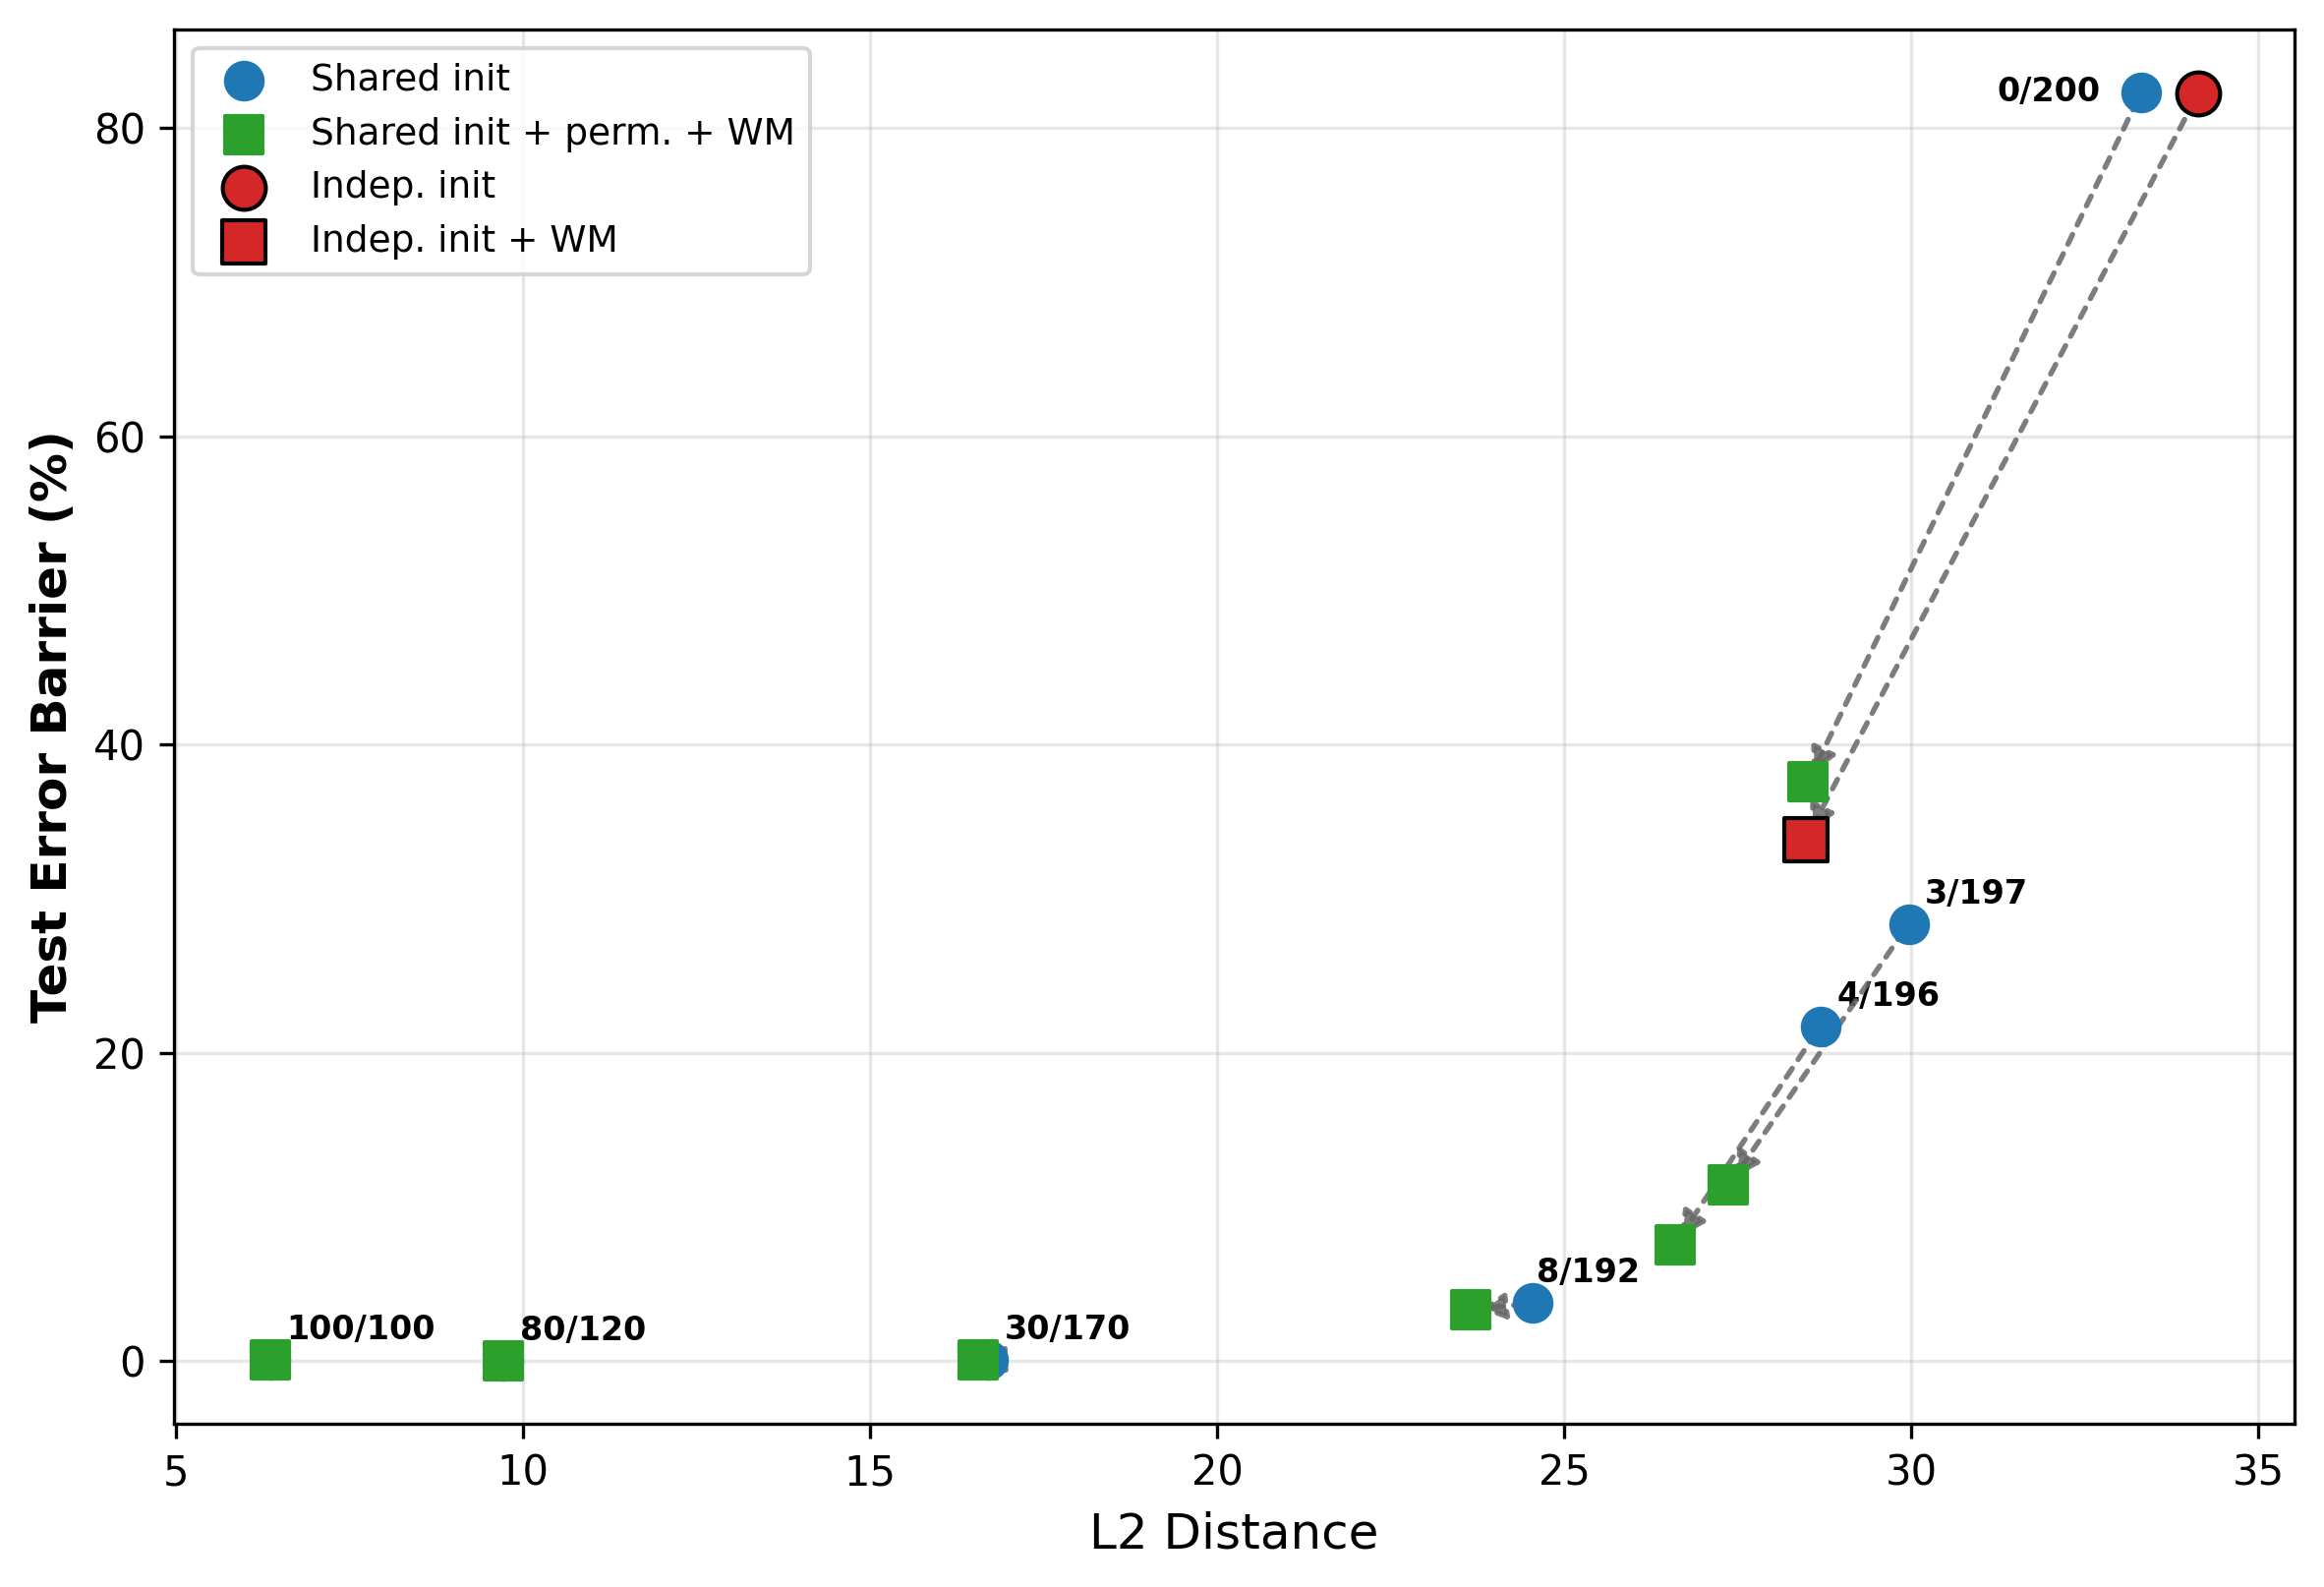
\includegraphics[width=0.94\linewidth]{test_error_acc_nonrel.png}
    \caption{VGG16/CIFAR-10 shared-training benchmark.  Labels $n/(200-n)$
    denote shared/independent epochs.  Circles are original endpoints; squares
    are endpoints after applying a random permutation and weight matching.
    Red denotes independent initialization.  Later splits remain closer and
    have lower barriers after alignment.}
    \label{fig:training-stage}
\end{figure}

\section{VGG/CIFAR-10 Validation}
\label{sec:vgg}

Figure~\ref{fig:vgg} reports test-loss barriers for four VGG architectures.
Permutation-only Sinkhorn reduces the raw barriers from roughly $1.88$--$1.98$
to $0.38$, $0.79$, $1.22$, and $1.21$ for VGG11/13/16/19.  Adding scales
improves on permutation-only in every architecture.  The better of joint and
sequential scaling attains $0.109$, $0.429$, $1.035$, and $1.105$,
respectively.  Relative to permutation-only, these are reductions of about
$71\%$, $45\%$, $15\%$, and $9\%$.

Neither optimization order dominates.  Joint permutation+scale is better for
VGG11 and VGG19; freezing the permutation and refining scales is better for
VGG13 and VGG16.  This echoes XOR: the symmetry class contains better
representatives, but joint nonconvex optimization does not always realize the
full gain.  Substantial barriers also remain for deeper VGGs, so permutation
and scale together are not a complete account of LMC.

The VGG results should be read as a transfer check of the controlled XOR
finding.  Exhaustive permutation search is impossible, only one endpoint pair
is used per architecture, and hyperparameters are selected per method.
Nevertheless, the consistent direction of change across four architectures
supports the practical relevance of scaling beyond the toy setting.

\begin{figure}[t]
    \centering
    \includegraphics[width=\linewidth]{barplot_vggs.png}
    \caption{Maximum test-loss barrier for independently trained VGG models on
    CIFAR-10.  Both scale-aware variants improve on Sinkhorn permutation-only
    for all four fixed endpoint pairs, although joint and sequential
    optimization trade places across architectures.}
    \label{fig:vgg}
\end{figure}

\section{Discussion and Limitations}

\paragraph{A refined one-basin picture.}
Our experiments separate three claims that are easy to collapse into one.
First, curved connectivity can exist without a good straight path.  Second,
permutations can remove representational mismatch, but the exhaustive XOR
result shows that this exact symmetry is not always sufficient.  Third,
overparameterization can make both processes easier by supplying redundant
features and routes through function space.  Positive scale adds another exact
degree of freedom and systematically improves the oracle permutation, but does
not eliminate every barrier.  The evidence therefore favors connectivity
modulo a richer symmetry class over a literal permutation-only one-basin claim.

\paragraph{Optimization versus existence.}
The exhaustive protocol is central to this interpretation.  Without it, a high
barrier after Sinkhorn or weight matching could always be ascribed to search
failure.  Conversely, the gap between joint Sinkhorn and oracle refinement
warns against treating a failed continuous relaxation as evidence that a good
monomial representative does not exist.  Future work should distinguish the
expressivity of a transformation class from the solver used to search it.

\paragraph{A diagnostic hierarchy for alignment failures.}
The experiments suggest a practical order for interpreting a residual barrier.
First, establish whether search error can be removed.  Exhaustive enumeration
is available only for small networks, but multiple restarts, exact matching in
restricted layers, or controlled known-permutation benchmarks can still reveal
optimizer limitations.  Second, if the best permutation remains inadequate,
expand the exact symmetry class before concluding that modes occupy distinct
basins.  Scale refinement is useful here because it is continuous, function
preserving after the permutation is fixed, and can be attached to existing
aligners.  Third, compare linear alignment with nonlinear paths and width
changes.  A curved path that appears after adding a unit is evidence for
representational slack, not evidence that a hidden permutation was recovered.
This hierarchy separates what transformation exists, whether an algorithm finds
it, and whether the architecture has enough redundancy for the desired path.

For model merging, the results also favor a direct validation rule: endpoint
equivalence should be checked after every transformation, and the full
interpolation profile should be measured on held-out data.  Small Euclidean
distance is not by itself a certificate of compatibility, as the training-stage
experiment demonstrates.  Conversely, a scale-aware transformation can
redistribute parameter differences while lowering the loss barrier.  Objectives
designed for merging should therefore target functional behavior along the
path, using weight distance only as a computational proxy.

\paragraph{Limitations.}
The exact conclusions come from small one-hidden-layer XOR networks.  The VGG
study is non-exhaustive, uses a single pair per architecture, and relies on
method-specific hyperparameter selection.  Our nonlinear path searches can
certify found paths but cannot certify nonexistence.  The scale-aware soft
transformation is exactly function preserving only after projection; during
Sinkhorn optimization it is a relaxation.  Finally, we consider ReLU networks,
for which positive homogeneity holds, and do not address normalization layers,
residual architectures, attention symmetries, or approximate functional
equivalences.  Larger multi-seed studies and comparisons with activation repair
are needed before drawing broad architectural conclusions.

\section{Conclusion}

Permutation symmetry is an important but incomplete explanation of linear mode
connectivity.  Exhaustive XOR search exposes genuine permutation-only failures;
increasing width rapidly suppresses them and changes nonlinear connectivity;
and positive scaling improves even the best possible permutation.  The same
directional gain appears in VGG/CIFAR-10, while a shared-training experiment
shows how alignment difficulty grows as optimization trajectories diverge.
Together, the results suggest that the useful object is not a basin modulo
permutation alone, but a low-loss geometry shaped jointly by exact symmetries,
width, and the history of optimization.

\subsection*{AI use statement}
Generative AI tools were used to discuss ideas, improve the organization and
clarity of draft text, and assist with programming tasks including debugging,
refactoring, plotting, and \LaTeX{} editing.  The research questions,
experimental design, implementation decisions, analysis, and conclusions were
determined by the authors.  AI-assisted text and code were reviewed and checked
before inclusion.  The authors take responsibility for the final content,
claims, citations, and artifacts.  This statement should be reconciled with the
final author team's use before submission.

\bibliography{references}
\bibliographystyle{iclr2027_conference}

\appendix

\section{Reproducibility Details}
\label{app:details}

\subsection{XOR training and exhaustive alignment}

The XOR set is $\{(0,0),(0,1),(1,0),(1,1)\}$ with labels
$\{0,1,1,0\}$.  Models have one ReLU hidden layer, biases, and one output logit.
Full-batch SGD uses learning rate $0.05$ and at most $5000$ epochs.
\texttt{ReduceLROnPlateau} uses factor $0.5$, patience $200$, threshold
$10^{-4}$, and minimum learning rate $5\times10^{-4}$.  Training stops when
loss has not improved by $10^{-4}$ for $500$ epochs.  For each retained pair,
all $h!$ permutations are evaluated.  Interpolation selection prioritizes
classification error in the width-$2$ diagnostic and loss barrier in the
scale-aware study.

For nonlinear paths, both quadratic B\'ezier curves and polygonal chains are
optimized for $1500$ steps at learning rate $0.05$, with no weight decay and
$31$ path samples.  The default path has one trainable interior point; harder
pairs use up to ten.

\subsection{XOR scale-aware optimization}

Final interpolation curves use $61$ evaluation points; optimization uses $31$
points.  The default permutation-only Sinkhorn run uses Adam for $500$ steps,
learning rate $0.01$, temperature $1$, $20$ Sinkhorn iterations, and identity
strength $1$.  Scale refinement uses Adam for $500$ steps, learning rate
$0.01$, and log-scale regularization $10^{-3}$.  Joint optimization uses the
same default budget.  If a default run misses its target, a bounded search over
learning rates, temperatures, and regularization is used; settings are selected
per pair.  The scale target is barrier $\epsilon=0.01$, while permutation-only
Sinkhorn targets that pair's exhaustive barrier.

\subsection{VGG experiments}

The shared-training benchmark follows a 200-epoch VGG16/CIFAR-10 schedule.
Branches differ in minibatch order and stochastic augmentation after the split.
The artificial full-network permutation uses seed 42; weight matching uses at
most 100 block-coordinate iterations and is repeated with three layer-update
orders.

For the scale-aware comparison, fixed seed-0/seed-1 endpoint pairs are used for
VGG11/13/16/19.  Alignment uses a deterministic batch of $1000$ images, 20
Sinkhorn iterations, and midpoint loss.  Separate bounded sweeps select the
number of optimization steps, learning rate, temperature, and scale
regularization for each architecture and method.  The permutation-then-scale
baseline freezes the projected hard permutation and optimizes only log-scales.

\section{Additional Pairwise Results}

Table~\ref{tab:pairwise} separates the practical optimization gap from the gain
provided by the symmetry class.  Sinkhorn permutation-only exactly matches the
exhaustive oracle on progressively fewer pairs as width grows.  Joint
permutation+scale often beats the permutation oracle, but oracle scale
refinement is the most reliable condition.

\begin{table}[h]
\caption{Pairwise XOR comparisons.  Lower loss barrier is better.}
\label{tab:pairwise}
\centering
\small
\begin{tabular}{lccc}
\toprule
Comparison & $h=3$ & $h=5$ & $h=7$ \\
\midrule
Oracle+scale $\leq$ oracle permutation & $21/21$ & $36/36$ & $10/10$ \\
Joint permutation+scale $\leq$ oracle permutation & $9/21$ & $29/36$ & $8/10$ \\
Sinkhorn permutation $=$ oracle permutation & $9/21$ & $7/36$ & $0/10$ \\
Oracle+scale $\leq$ joint permutation+scale & $15/21$ & $25/36$ & $5/10$ \\
\bottomrule
\end{tabular}
\end{table}

\end{document}
